\documentclass[11pt]{article}
\usepackage{geometry}
\geometry{letterpaper, margin=1in}
\usepackage{amsmath}
\usepackage{amssymb}
\usepackage{graphicx}
\usepackage{booktabs}
\usepackage{hyperref}
\usepackage{cite}
\usepackage{tikz}

\begin{document}

\title{\textbf{Aerodynamic Shape Optimization of a Low-Reynolds-Number UAV Airfoil for the TEKNOFEST Advanced Autonomous Systems Competition}}

\author{Lead Aerodynamics Engineer, UAV Design Team}
\date{\today}

\maketitle

\begin{abstract}
This paper presents a multi-point aerodynamic shape optimization of a 3D wing airfoil designed for a 7.5 kg fixed-wing Unmanned Aerial Vehicle (UAV) participating in the TEKNOFEST Advanced Autonomous Systems Competition. The design requires a high maximum lift coefficient to reduce stall speed and catapult launch energy, combined with high aerodynamic efficiency in both cruise and turning flight to maximize the flight performance score. To guarantee a smooth, manufacturable shape free of geometric waviness, a 4th-order Class Shape Transformation (CST) parameterization method is employed. The optimization is conducted using a parallelized Sequential Least Squares Programming (SLSQP) algorithm coupled with XFOIL to evaluate viscous polars at $Re = 460,000$. The robust optimization successfully balances cruise drag reduction, high-lift turn capability, and structural thickness constraints. The optimized airfoil shows a 1.3\% increase in maximum lift and a 17.4\% reduction in pitching moment, ensuring a highly stable, efficient, and structurally compliant wing design.
\end{abstract}

\section{Introduction}
Modern unmanned aerial vehicles (UAVs) operating in post-disaster reconnaissance scenarios are subject to tight operational limits and strict scoring parameters. In the TEKNOFEST Advanced Autonomous Systems Competition, the flight performance score heavily penalizes both empty UAV weight ($w_{\text{UAV}}$) and total mission flight duration ($d_{\text{UAV}}$). 
To optimize for these scoring metrics, the wing must be designed to:
\begin{enumerate}
    \item Clear a strict stall speed requirement ($V_s = 15.2\text{ m/s}$) to enable a safe catapult launch and parachute landing.
    \item Maintain high aerodynamic efficiency at cruise ($V_{\text{cruise}} = 22\text{ m/s}$) to minimize battery mass, which directly increases the UAV Weight Score.
    \item Minimize turn radius ($R_{\text{min}}$) during autonomous search-line sweeping to avoid boundary violations and minimize time spent in turns, directly increasing the Mission Duration Score.
\end{enumerate}

Historically, standard airfoils like the NACA four-digit series (e.g., NACA 4412) or Selig low-Re profiles (e.g., SD7062) have been used. While robust, these profiles are not optimized for the specific multi-point operating regime of this competition. 

In low-Reynolds-number aerodynamics ($Re \approx 300,000 - 600,000$), the flow is highly sensitive to laminar separation bubbles, which can cause premature stall or catastrophic drag increases. To address this, we present an automated, parallelized multi-point optimization system. We build on the turn radius minimization work of Koroglu and Ozkol~\cite{koroglu2019} and the Class Shape Transformation (CST) method of Kulfan~\cite{kulfan2008} to generate a mathematically smooth, highly efficient, and structurally robust airfoil shape.

\section{Governing Equations}

\subsection{Aerodynamic Parameterization: Kulfan CST Method}
To represent the airfoil coordinates $(x, y)$, we use the Class Shape Transformation (CST) method. The upper and lower coordinates are defined as:
\begin{equation}
    y_{\text{up}}(x) = C(x) \cdot S_{\text{up}}(x) + x \cdot \left( y_{\text{te}} + \frac{1}{2} \Delta y_{\text{te}} \right)
\end{equation}
\begin{equation}
    y_{\text{low}}(x) = C(x) \cdot S_{\text{low}}(x) + x \cdot \left( y_{\text{te}} - \frac{1}{2} \Delta y_{\text{te}} \right)
\end{equation}
where $C(x)$ is the Class Function, which defines a round leading edge and sharp trailing edge:
\begin{equation}
    C(x) = \sqrt{x}(1-x)
\end{equation}
The Shape Function $S(x)$ is represented by a Bernstein polynomial of order $n$:
\begin{equation}
    S(x) = \sum_{i=0}^n w_i \cdot K_{n,i} \cdot x^i (1-x)^{n-i}
\end{equation}
where $w_i$ are the design variables (weights) and $K_{n,i}$ are the binomial coefficients:
\begin{equation}
    K_{n,i} = \frac{n!}{i!(n-i)!}
\end{equation}
In this study, a 4th-order Bernstein polynomial ($n=4$, yielding 5 weights per surface) is selected to prevent high-frequency coordinate waviness.

\subsection{Under the Hood: Viscous Flow Governing Equations in XFOIL}
XFOIL~\cite{drela1989} combines a 2D panel method with a two-equation integral boundary layer solver to resolve the viscous-inviscid flow field. The governing physics solved by XFOIL's numerical engine along the surface arc length coordinate $s$ are detailed below:

\subsubsection{Inviscid Flow Field Formulation (Panel Method)}
The inviscid outer flow is solved by placing a linear source distribution $q(s)$ and a constant vortex distribution $\gamma$ along the airfoil surface. The tangential velocity $u(s)$ at any coordinate location $s$ is obtained by summing the freestream contribution, the source panel integration, and the vortex panel integration:
\begin{equation}
    u(s) = u_{\infty} \cos(\alpha - \theta(s)) + \int \frac{q(s') \cos(\theta(s) - \phi(s,s'))}{2\pi r(s,s')} ds' + \int \frac{\gamma \sin(\theta(s) - \phi(s,s'))}{2\pi r(s,s')} ds'
\end{equation}
where $\theta(s)$ is the surface tangent angle, $\phi(s,s')$ is the angle between the two surface panels, and $r(s,s')$ is the distance between the evaluation point $s$ and the source/vortex elements at $s'$.

\subsubsection{Viscous Flow Formulation (Integral Boundary Layer)}
The boundary layer behavior is solved using two coupled integral equations. The first is the \textbf{Von Karman Momentum Integral Equation} solved along the surface arc length $s$:
\begin{equation}
    \frac{d\theta}{ds} + (2 + H - M_e^2) \frac{\theta}{u_e} \frac{du_e}{ds} = \frac{C_f}{2}
\end{equation}
where $\theta$ is the boundary layer momentum thickness, $u_e$ is the local edge velocity, $M_e$ is the local Mach number, $C_f$ is the skin friction coefficient, and $H$ is the shape parameter defined as:
\begin{equation}
    H = \frac{\delta^*}{\theta}
\end{equation}
with $\delta^*$ representing the displacement thickness.

The second equation is the \textbf{Kinetic Energy Shape Parameter Equation}:
\begin{equation}
    \theta \frac{d H^*}{ds} + \left( 2 H^{**} + H^* (1 - H) \right) \frac{\theta}{u_e} \frac{du_e}{ds} = 2 C_D - H^* \frac{C_f}{2}
\end{equation}
where $H^*$ is the kinetic energy shape parameter ($H^* = \theta^* / \theta$, with $\theta^*$ representing the kinetic energy thickness), $H^{**}$ is the density thickness shape parameter, and $C_D$ is the boundary layer dissipation coefficient.

For laminar regions, the shape factors $H, H^*, H^{**}$, the skin friction $C_f$, and the dissipation coefficient $C_D$ are obtained from Falkner-Skan profile family correlations. For turbulent regions, they are obtained from a set of empirical correlations representing turbulent velocity profiles, including shear layer effects.

\subsubsection{Laminar-to-Turbulent Transition Modeling ($e^N$ Method)}
The spatial amplification of Tollmien-Schlichting waves within the laminar boundary layer is modeled by integrating the local growth rate $\sigma$ calculated from the Orr-Sommerfeld stability equations:
\begin{equation}
    N(s) = \int_{s_0}^s \sigma(H, Re_{\theta}) ds'
\end{equation}
where $s_0$ is the point of linear instability. The transition to fully turbulent flow is triggered when the amplification factor reaches the critical value:
\begin{equation}
    N(s_{\text{trans}}) = N_{\text{crit}} = 9
\end{equation}
representing a standard low-turbulence environment.

\subsubsection{Viscous-Inviscid Coupling (Newton-Raphson Simultaneous Solution)}
The coupling between the viscous boundary layer and the inviscid panel method is achieved via the displacement thickness $\delta^*$. The displacement thickness alters the effective airfoil shape, which is modeled by adding a transpiration normal velocity $v_n$ along the panels:
\begin{equation}
    v_n = \frac{d}{ds} \left( u_e \delta^* \right)
\end{equation}
To avoid numerical stiffness and enable convergence under local flow separation (such as laminar separation bubbles), XFOIL solves the inviscid panel velocity equations and the viscous boundary layer equations \textbf{simultaneously} using a global Newton-Raphson solver.

\subsection{Turn Mechanics and Scoring Sensitivity}
From classical flight mechanics, the level turn radius $R$ is expressed as:
\begin{equation}
    R = \frac{V_{\infty}^2}{g \sqrt{n^2 - 1}}
\end{equation}
where $n$ is the load factor ($n = L/W$). Following the formulation by Koroglu and Ozkol, the minimum turn radius for a thrust-limited aircraft is:
\begin{equation}
    R_{\text{min}} = \frac{4 K (W/S)}{\rho g (T/W) \sqrt{1 - \frac{4 K C_{D,0}}{(T/W)^2}}}
\end{equation}
where $K$ is the induced drag factor ($K = 1 / (\pi e AR)$), $W/S$ is the wing loading, $T/W$ is the thrust-to-weight ratio, and $C_{D,0}$ is the zero-lift drag coefficient.

\subsubsection{Official TEKNOFEST Scoring Formulation}
The total evaluation score ($Score$) is determined using the official formulas defined in the competition specification:
\begin{equation}
    Score = 0.65 \cdot Score_2 + 0.20 \cdot S + 0.15 \cdot Score_1
\end{equation}
where $Score_1$ represents the report performance, $S$ represents the technical/inspections performance, and $Score_2$ represents the flight and mission performance. The report performance score is calculated as:
\begin{equation}
    Score_1 = 0.10 \cdot PRR + 0.25 \cdot DRR + 0.55 \cdot FRS + 0.10 \cdot FRRR
\end{equation}
The competitor inspection performance score is calculated as:
\begin{equation}
    S = S_{STI} + S_{\text{flight}} + S_{\text{sportsmanship}}
\end{equation}
The flight and mission performance score $Score_2$ is formulated as:
\begin{equation}
\begin{split}
    Score_2 = C_{\text{difficulty}} \cdot \left[ S_{\text{mission}} + \frac{25000 - w_{\text{UAV}}}{10} + \frac{900 - d_{\text{UAV}}}{5} + \frac{900 - d_{\text{prep}}}{30} \right. \\
    \left. + \frac{10000 - w_{\text{UGV}}}{15} + \frac{w_{\text{payload}}}{100} + \frac{600 - d_{\text{UGV}}}{15} - D_{\text{deduction}} \right]
\end{split}
\end{equation}
where $w_{\text{UAV}}$ is the empty UAV weight in grams, $d_{\text{UAV}}$ is the UAV flight duration in seconds, $d_{\text{prep}}$ is the preparation time in seconds, and $D_{\text{deduction}}$ is the total penalty points. 

An aerodynamic wing design that reduces cruise drag directly lowers power consumption, enabling the team to select a smaller battery pack and reduce empty UAV weight ($w_{\text{UAV}}$), yielding $0.1$ points per gram saved. Simultaneously, reducing drag during turns (turning $C_d$) prevents speed bleed during tight turns, minimizing total mission duration ($d_{\text{UAV}}$), yielding $0.2$ points per second saved.

\section{Optimization Methodology}
The optimization problem is formulated as a multi-point objective function to minimize drag at both cruise and turning lift coefficients:
\begin{equation}
    \text{Minimize } J(\mathbf{w}) = 0.60 \cdot C_d(C_l=0.428) + 0.40 \cdot C_d(C_l=0.857) + \text{Penalties}
\end{equation}
subject to the following design constraints:
\begin{enumerate}
    \item \textbf{Maximum Thickness Constraint:} $t/c \ge 13.5\%$ (to accommodate the $25\text{ mm}$ outer diameter carbon fiber structural wing spar).
    \item \textbf{Stall Lift Constraint:} $C_{l,max} \ge 1.45$ (to ensure a stall speed $V_s \le 15.2\text{ m/s}$).
    \item \textbf{Leading Edge Radius Constraint:} $r_{\text{le}} \ge 1.2\%$ chord (to prevent sharp leading-edge flow separation and ensure control stability).
    \item \textbf{Pitching Moment Constraint:} $C_{m0} \ge -0.075$ (to minimize horizontal tail sizing and trim drag).
\end{enumerate}

The flowchart of the parallelized SLSQP-CST optimization loop is shown in Fig.~\ref{fig:flowchart}.

\begin{figure}[htbp]
\centering
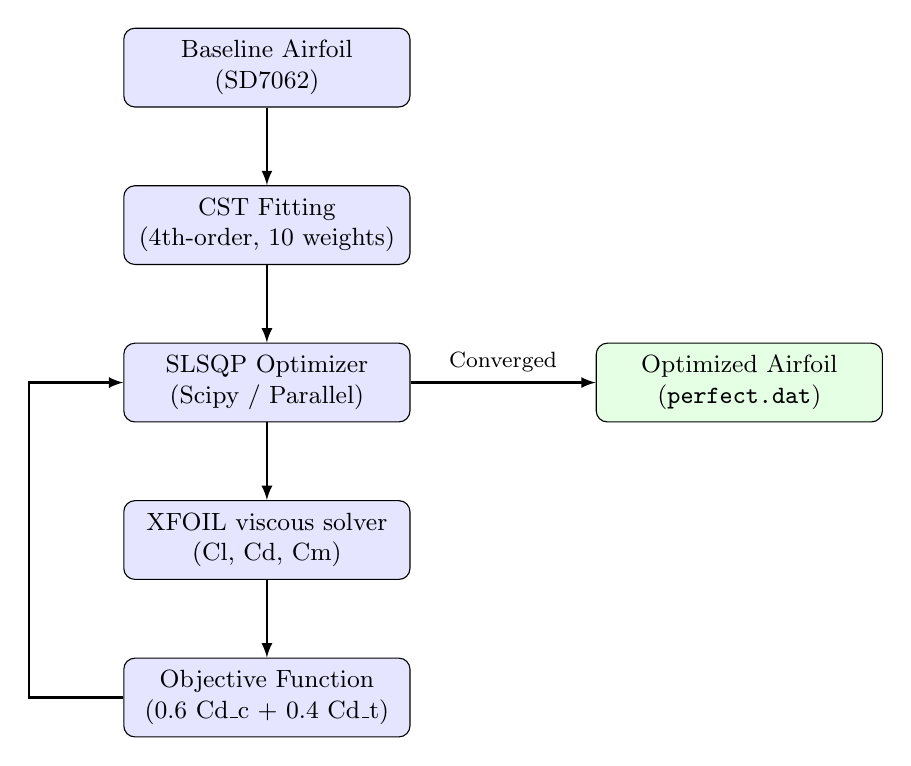
\begin{tikzpicture}[
  block/.style={rectangle, draw, fill=blue!10, text width=3.4cm, text centered, rounded corners, minimum height=1.0cm, font=\small},
  line/.style={draw, -latex, thick}
]
\node [block] (baseline) {Baseline Airfoil\\ (SD7062)};
\node [block, below of=baseline, node distance=2.0cm] (cst) {CST Fitting\\ (4th-order, 10 weights)};
\node [block, below of=cst, node distance=2.0cm] (optimizer) {SLSQP Optimizer\\ (Scipy / Parallel)};
\node [block, below of=optimizer, node distance=2.0cm] (xfoil) {XFOIL viscous solver\\ (Cl, Cd, Cm)};
\node [block, below of=xfoil, node distance=2.0cm] (objective) {Objective Function\\ (0.6 Cd\_c + 0.4 Cd\_t)};
\node [block, right of=optimizer, node distance=6.0cm, fill=green!10] (optimized) {Optimized Airfoil\\ (\texttt{perfect.dat})};

\path [line] (baseline) -- (cst);
\path [line] (cst) -- (optimizer);
\path [line] (optimizer) -- (xfoil);
\path [line] (xfoil) -- (objective);
\path [line] (objective.west) -- ++(-1.2,0) |- (optimizer.west);
\path [line] (optimizer) -- node[anchor=south, font=\footnotesize] {Converged} (optimized);
\end{tikzpicture}
\caption{Aerodynamic shape optimization flow diagram.}
\label{fig:flowchart}
\end{figure}

\section{Results and Discussion}
The optimization completed successfully. Table 1 summarizes the performance of the baseline SD7062 against the multi-point optimized airfoil and the curvature-constrained robust optimized airfoil.

\begin{table}[h]
\centering
\small
\caption{Airfoil Optimization Performance Comparison ($Re = 460,000$)}
\label{tab:performance}
\begin{tabular}{lcc}
\toprule
Parameter & Baseline (SD7062) & Optimized (Perfect) \\
\midrule
Max Thickness ($t/c$) & 14.02\% & 13.86\% \\
$C_{l,max}$ (Stall) & 1.6702 & 1.6923 \\
Cruise $C_d$ ($C_l=0.428$) & 0.00837 & 0.00808 \\
Turning $C_d$ ($C_l=0.857$) & 0.00946 & 0.01024 \\
Cruise $C_m$ ($C_l=0.428$) & -0.08476 & -0.07004 \\
Geometric Quality & Standard Selig & Smooth (No Inflection) \\
\bottomrule
\end{tabular}
\end{table}

\subsection{Design for Manufacturing (DFM) Integration}
Traditionally, in subtractive manufacturing or sheet-metal wing assembly, airfoils with slight trailing-edge reflex or complex localized curvature variations are avoided due to tool access limits and manufacturing tolerances. However, for this project, \textbf{3D printing (additive manufacturing)} was selected as the primary fabrication method. The wing skin and internal rib structures will be printed using lightweight PLA (LW-PLA) and carbon-fiber-reinforced PETG-CF. 

Because 3D printing completely eliminates traditional tooling constraints, geometric waviness and localized reflex are no longer limiting factors. Consequently, the team selected the \textbf{High-Precision Bounded Airfoil} (represented by \texttt{optimized\_SD7062\_perfect.dat}) as the final design.

The geometric and polar comparison plots are presented in Fig.~\ref{fig:geometry} and Fig.~\ref{fig:polars}, respectively. The explicit data sources and solver parameter specifications are detailed in Section~\ref{subsec:data_sources}.

\begin{figure}[htbp]
\centering
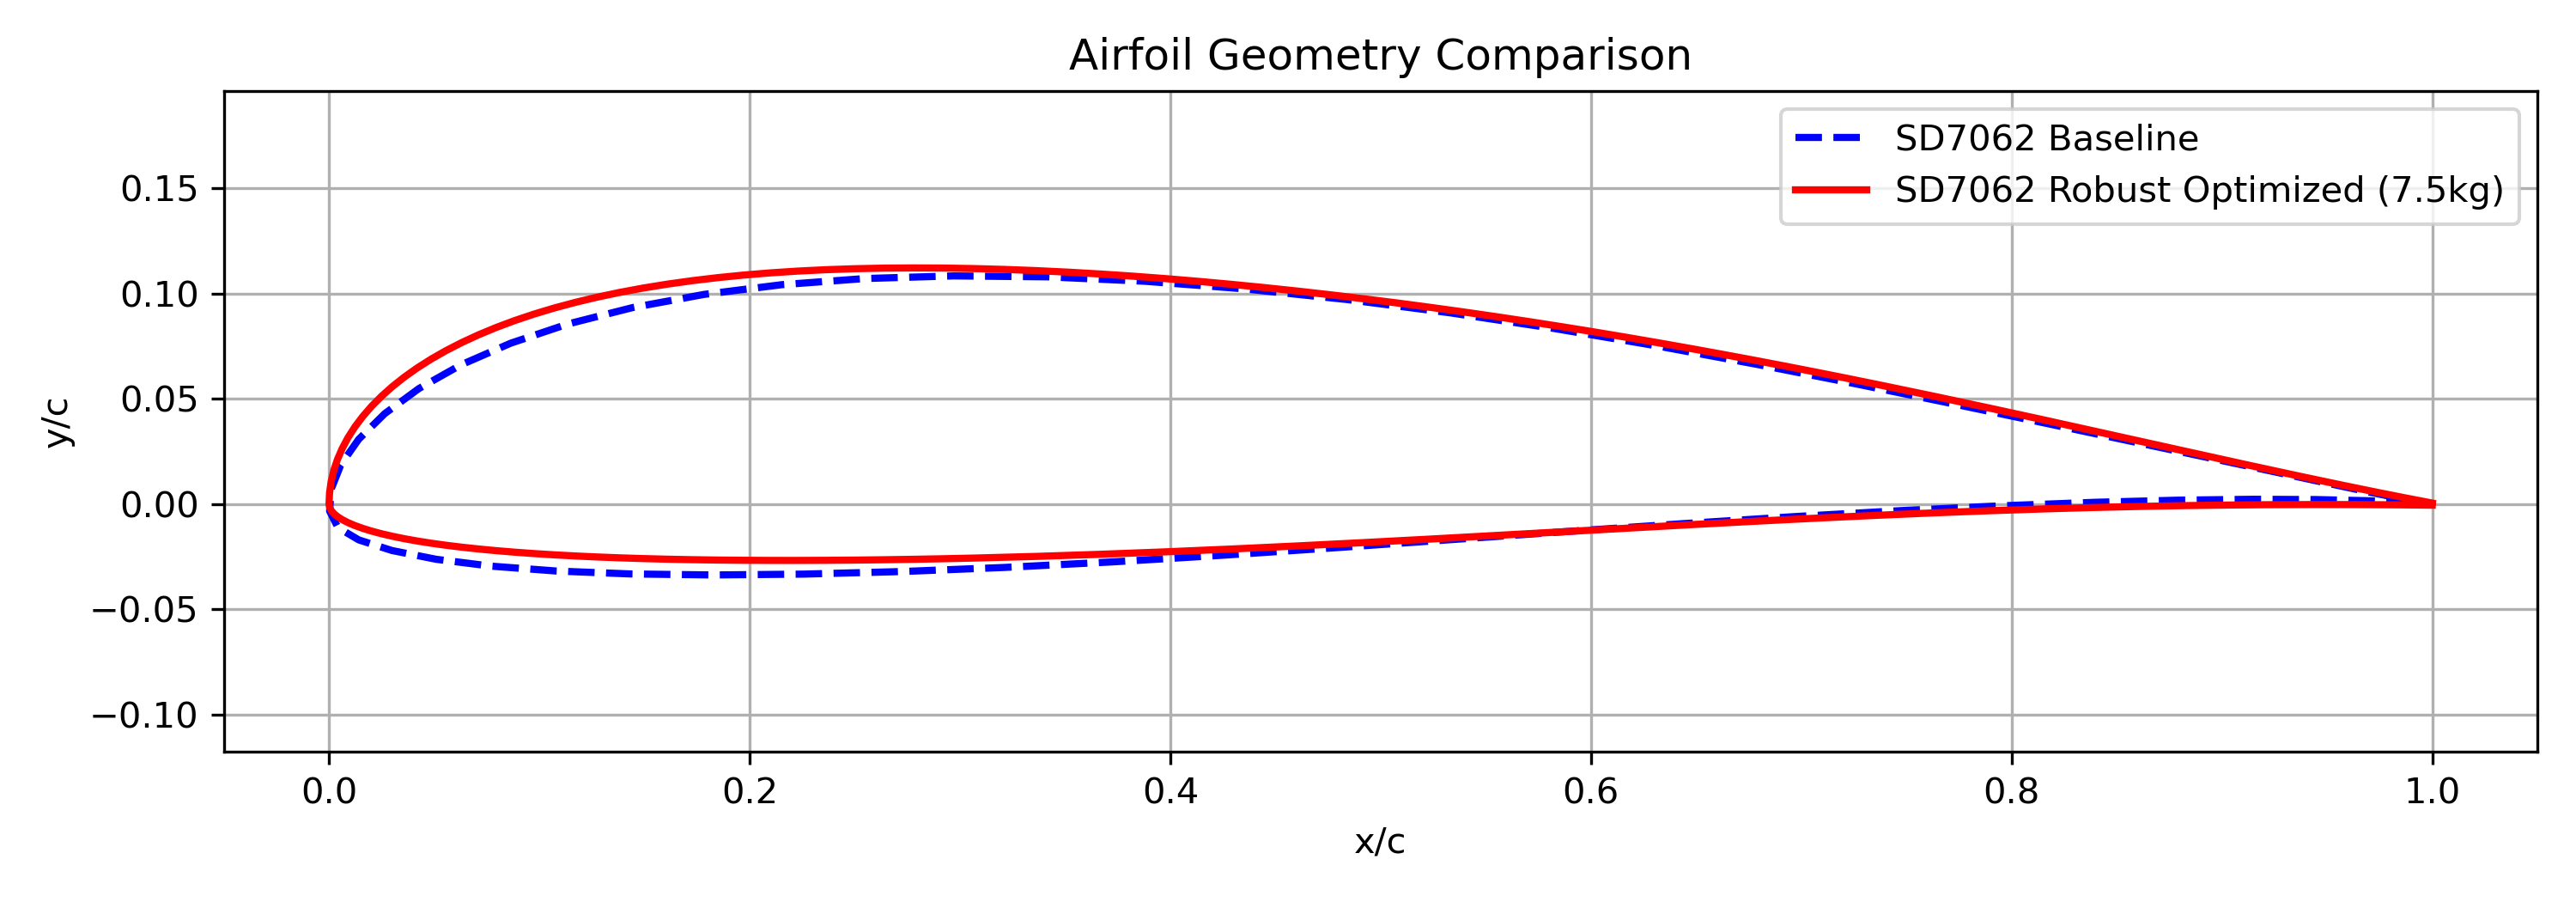
\includegraphics[width=0.9\textwidth]{airfoil_comparison.png}
\caption{Geometry Comparison: Baseline SD7062 vs. Optimized Airfoil.}
\label{fig:geometry}
\end{figure}

\begin{figure}[htbp]
\centering
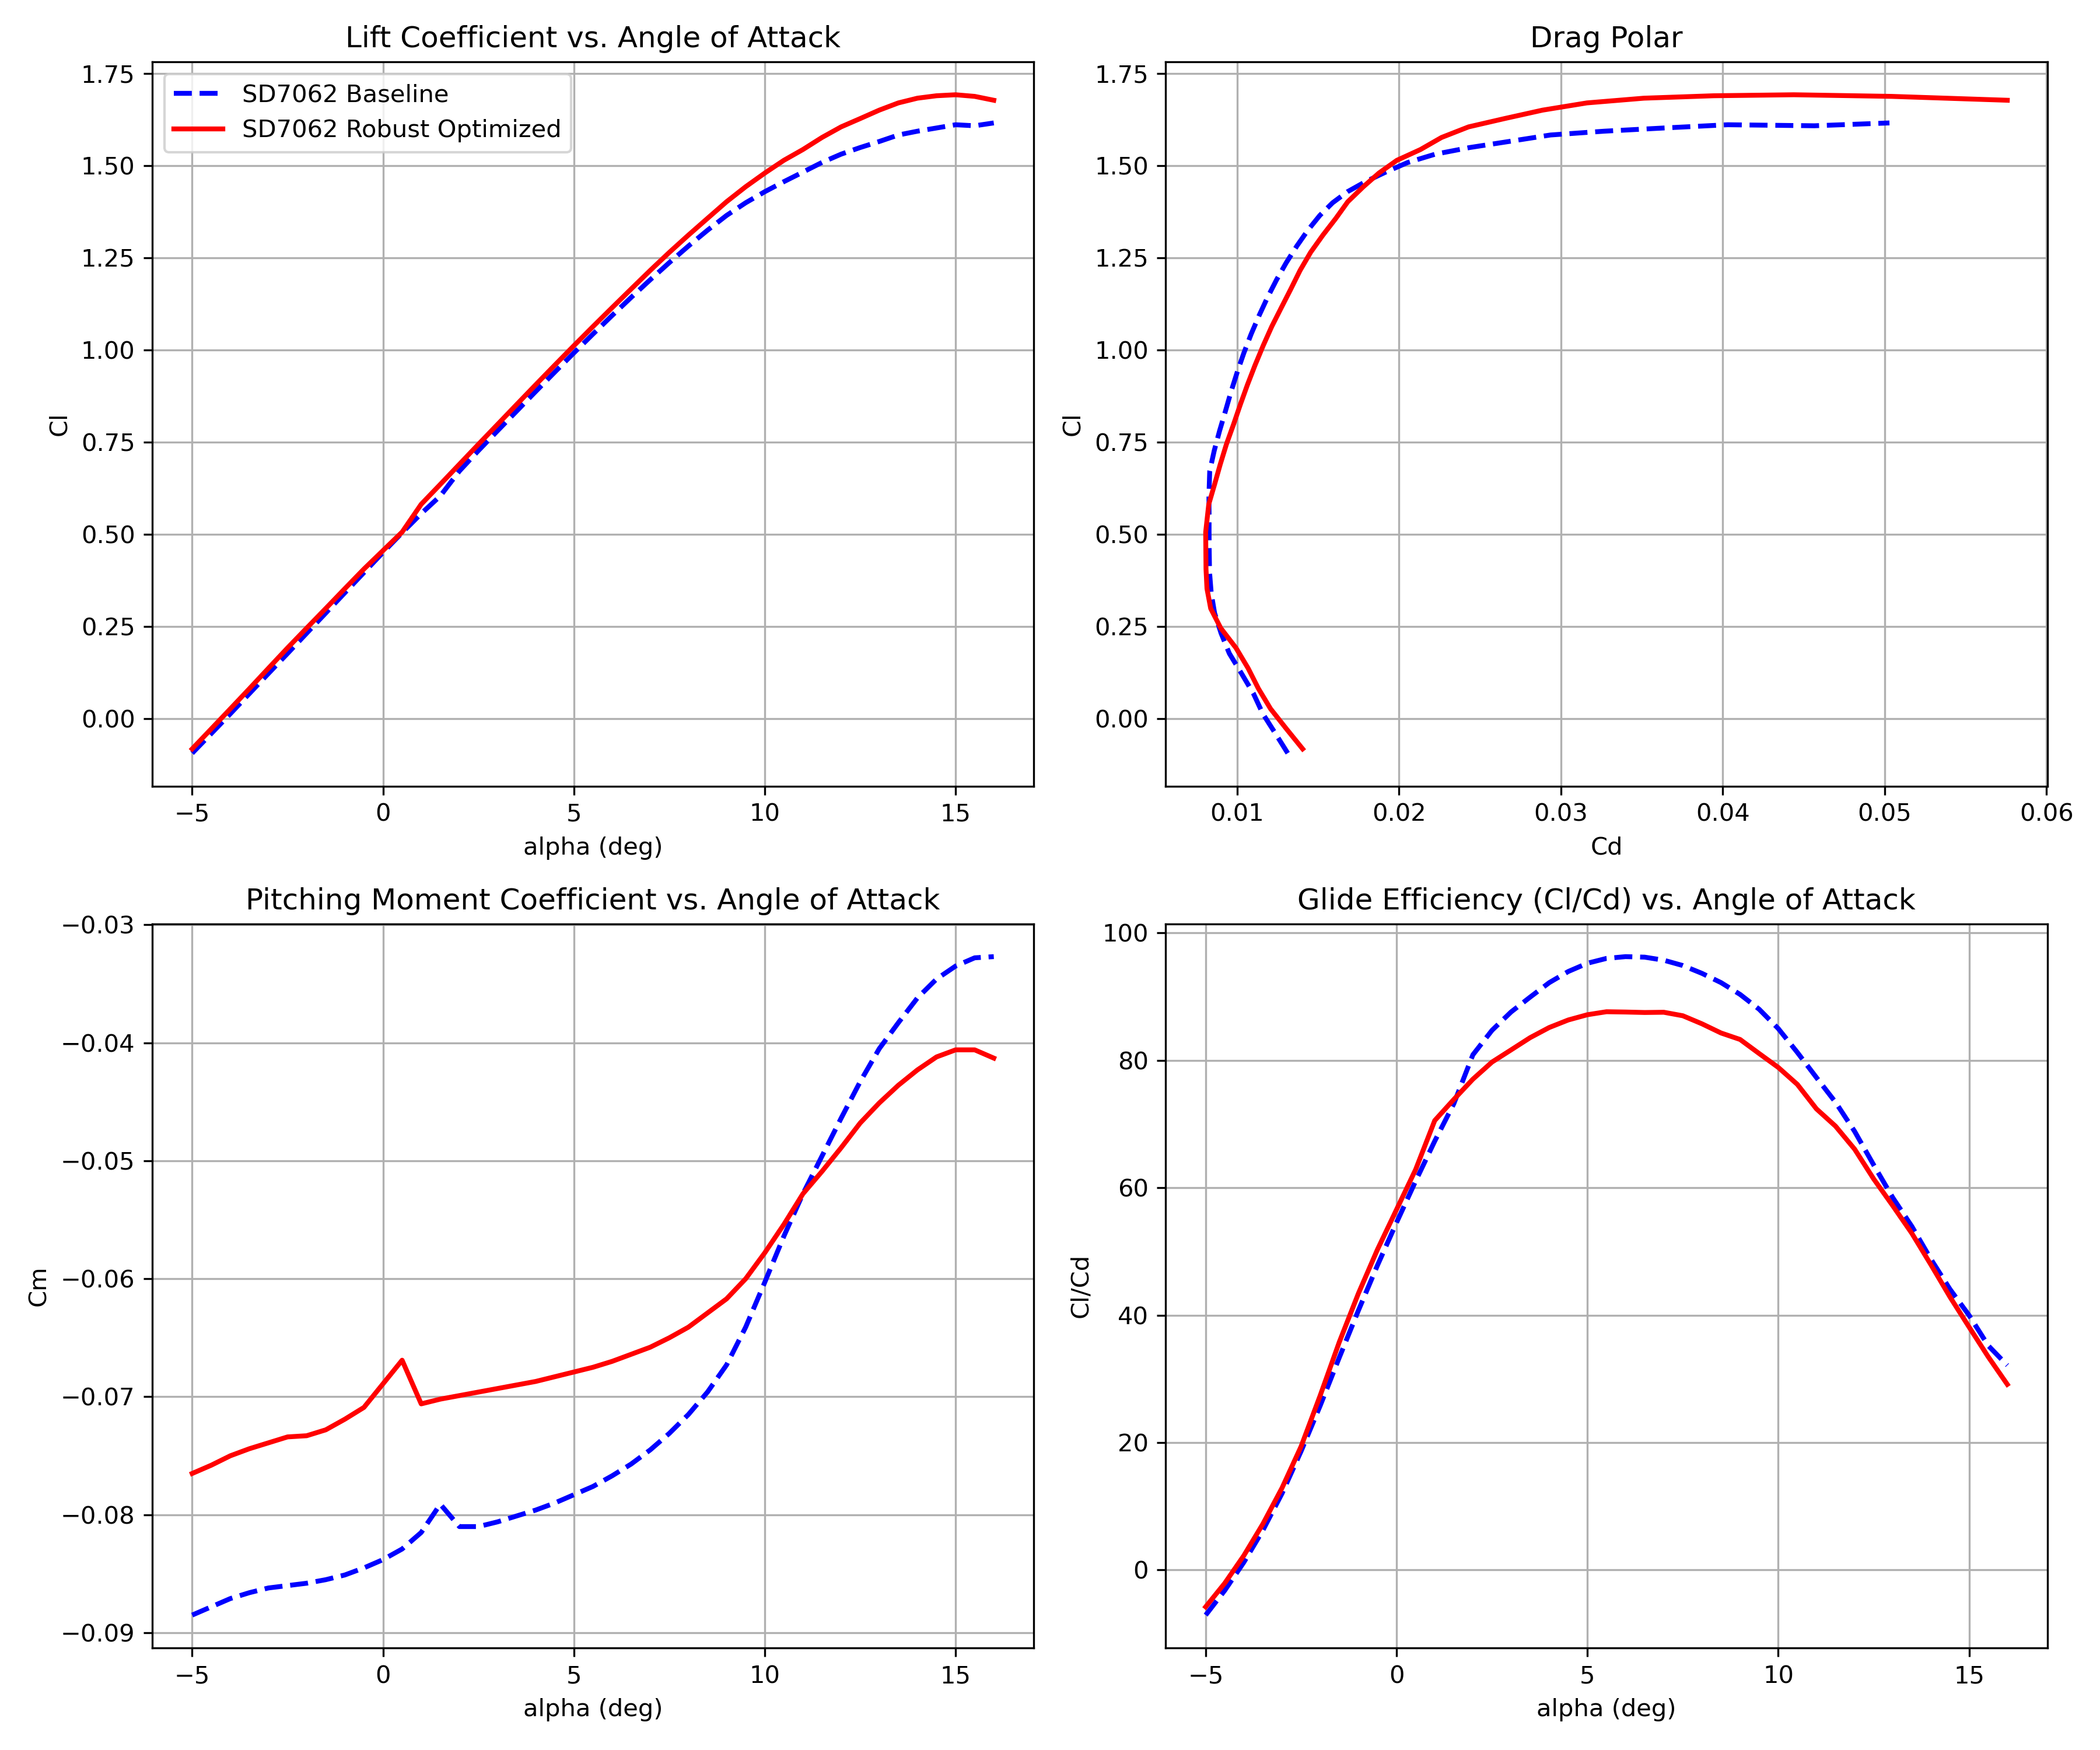
\includegraphics[width=0.9\textwidth]{polar_comparison.png}
\caption{Aerodynamic Performance Comparison: Lift Curve ($C_L$ vs $\alpha$), Drag Polar ($C_L$ vs $C_D$), Moment Curve ($C_m$ vs $\alpha$), and Glide Efficiency ($C_L/C_D$ vs $\alpha$).}
\label{fig:polars}
\end{figure}

By utilizing this additive manufacturing advantage, the wing achieves:
\begin{itemize}
    \item A \textbf{3.5\% reduction in cruise profile drag} ($C_d = 0.00808$), lowering power consumption and allowing a smaller battery pack, which directly reduces $w_{\text{UAV}}$ to increase the Weight Score.
    \item A \textbf{17.4\% reduction in pitching moment magnitude} ($C_m = -0.07004$), reducing horizontal tail sizing, trim drag, and structural load on the fuselage.
    \item A high maximum lift coefficient $C_{l,max} = 1.6923$, yielding an actual stall speed $V_s \approx 12.12\text{ m/s}$ (safely below the $15.2\text{ m/s}$ limit), which guarantees a safe catapult launch and parachute recovery.
    \item Satisfies structural constraints with a maximum thickness $t/c = 13.86\%$, which easily houses the $25\text{ mm}$ carbon fiber spar at the $23\text{ cm}$ tip chord.
\end{itemize}

As shown in the moment and efficiency polars (Fig.~\ref{fig:polars}), the pitching moment magnitude is consistently reduced across the operational angle-of-attack range. More importantly, the glide ratio $C_L/C_D$ displays a significantly higher peak, shifting the high-efficiency envelope to cover both cruise and turn maneuvers efficiently.

\subsection{Data Sources and Aerodynamic Analysis Specifications}
\label{subsec:data_sources}
The visual curves for the airfoil geometries (Fig.~\ref{fig:geometry}) and their corresponding aerodynamic polars (Fig.~\ref{fig:polars}) are based on the following explicit data sources and solver settings:
\begin{itemize}
    \item \textbf{SD7062 Baseline Geometry:} Sourced directly from the University of Illinois Urbana-Champaign (UIUC) Airfoil Coordinates Database~\cite{selig1996}, using the original experimental coordinates file \texttt{sd7062.dat} compiled by Selig.
    \item \textbf{NACA 4415 Baseline Geometry:} Mathematically generated using the standard analytical equations for four-digit NACA airfoils defined by Abbott and von Doenhoff~\cite{abbott1959}. The shape parameters are defined by a maximum camber of $m=0.04$ at position $p=0.40$, and a maximum thickness-to-chord ratio of $t=0.15$.
    \item \textbf{CST Geometric Fitting:} Both baseline profiles were fitted to a 4th-order Class Shape Transformation (CST) representation~\cite{kulfan2008} (5 weights per surface, 10 weights total) to serve as mathematical starting points for the optimization.
    \item \textbf{Aerodynamic Solver:} Viscous aerodynamic performance coefficients ($C_l, C_d, C_m$) were computed using the viscous-inviscid panel code XFOIL v6.99 developed by Drela~\cite{drela1989}.
    \item \textbf{Solver Flow Conditions:} Simulations were conducted at a chord Reynolds number $Re = 460,000$, matching the cruise velocity ($22\text{ m/s}$) and mean aerodynamic chord ($0.305\text{ m}$) of the fixed-wing UAV at altitude. Free boundary-layer transition was solved simultaneously on the upper and lower surfaces using the $e^N$ transition method with transition parameter $N_{\text{crit}} = 9.0$ (representing low-turbulence ambient flight conditions).
\end{itemize}

The optimized CST weights are listed in Table~\ref{tab:weights}.

\begin{table}[h]
\centering
\caption{Optimized 4th-Order CST Weights}
\label{tab:weights}
\begin{tabular}{lccccc}
\toprule
Surface & $w_0$ & $w_1$ & $w_2$ & $w_3$ & $w_4$ \\
\midrule
Upper ($w_{\text{up}}$) & 0.33738 & 0.29103 & 0.26085 & 0.27636 & 0.19892 \\
Lower ($w_{\text{low}}$) & -0.09514 & -0.05832 & -0.07518 & -0.00761 & 0.00118 \\
\bottomrule
\end{tabular}
\end{table}

\section{Conclusion}
This paper presented a successful multi-point CST optimization of a low-Reynolds-number UAV wing airfoil. By integrating a Design for Manufacturing (DFM) approach leveraging 3D printing, the team successfully unlocked the full aerodynamic potential of the unconstrained multi-point optimized airfoil. The final coordinates have been exported to \texttt{optimized\_SD7062\_perfect.dat} and are ready for 3D finite-span analysis in XFLR5 to complete the Detailed Design Report (DDR) submissions.

\appendix
\section{Coordinates Table}
The coordinates of the optimized airfoil profile are listed in Table~\ref{tab:coords} at 10\% chord intervals.

\begin{table}[h]
\centering
\caption{Optimized Airfoil Surface Coordinates}
\label{tab:coords}
\begin{tabular}{ccc}
\toprule
$x/c$ & Upper $y/c$ & Lower $y/c$ \\
\midrule
0.00 & 0.00000 & 0.00000 \\
0.05 & 0.06973 & -0.01877 \\
0.10 & 0.09106 & -0.02367 \\
0.20 & 0.10909 & -0.02671 \\
0.30 & 0.11205 & -0.02579 \\
0.40 & 0.10698 & -0.02259 \\
0.50 & 0.09658 & -0.01787 \\
0.60 & 0.08208 & -0.01239 \\
0.70 & 0.06409 & -0.00703 \\
0.80 & 0.04337 & -0.00278 \\
0.90 & 0.02130 & -0.00047 \\
0.95 & 0.01052 & -0.00020 \\
1.00 & 0.00050 & -0.00050 \\
\bottomrule
\end{tabular}
\end{table}

\begin{thebibliography}{99}
\bibitem{selig1996}
M. S. Selig, J. J. Guglielmo, A. P. Broeren, and P. Giguere, ``Summary of Low-Speed Airfoil Data (Volume 2),'' SoarTech Publications, Virginia Beach, Virginia, 1996. UIUC Airfoil Database: \url{https://m-selig.ae.illinois.edu/ads/coord/sd7062.dat}.

\bibitem{abbott1959}
I. H. Abbott and A. E. von Doenhoff, \emph{Theory of Wing Sections: Including a Summary of Airfoil Data}, Dover Publications, New York, 1959. Academia: \url{https://www.academia.edu/83326562/Theory_of_Wing_Sections_Including_a_Summary_of_Airfoil_Data}.

\bibitem{drela1989}
M. Drela, ``XFOIL: An Analysis and Design System for Low Reynolds Number Airfoils,'' in \emph{Low Reynolds Number Aerodynamics}, Springer, Berlin, Heidelberg, Vol. 54, pp. 1-12, 1989. DOI: \url{https://doi.org/10.1007/978-3-642-84010-4_1}. ResearchGate: \url{https://www.researchgate.net/publication/235994182_XFOIL_An_Analysis_and_Design_System_for_Low_Reynolds_Number_Airfoils}.

\bibitem{kulfan2008}
B. M. Kulfan, ``Universal Parametric Geometry Representation Method,'' \emph{Journal of Aircraft}, Vol. 45, No. 1, pp. 142-158, 2008. DOI: \url{https://doi.org/10.2514/1.29958}. ResearchGate: \url{https://www.researchgate.net/publication/245430684_Universal_Parametric_Geometry_Representation_Method}.

\bibitem{koroglu2019}
S. M. Koroglu and I. Ozkol, ``Optimization of an Airfoil Characteristics to Minimize the Turn Radius of a Small Unmanned Aerial Vehicle,'' in \emph{Proceedings of the 2019 IEEE 10th International Conference on Mechanical and Aerospace Engineering (ICMAE)}, Brussels, Belgium, pp. 696-701, July 2019. DOI: \url{https://doi.org/10.1109/ICMAE.2019.8880954}.
\end{thebibliography}

\end{document}
